\documentclass[a4paper]{standalone}

% use this declaration to set specific page margins
%\usepackage[a4paper , lmargin = {2.7cm} , rmargin = {2.9cm} , tmargin = {2.7cm} , bmargin = {4.6cm} ]{geometry}
\usepackage[a4paper]{geometry}
\usepackage[ngerman, english]{babel}

\usepackage[utf8]{inputenc}
\usepackage[boxed]{algorithm2e}
\usepackage{amsmath}
\usepackage{amssymb}
\usepackage{authblk}
\usepackage{caption}
\usepackage{cleveref}
\usepackage [autostyle, english = american]{csquotes}
\usepackage{fontenc}
\usepackage{fontspec}
\usepackage{graphicx}
\usepackage[pagebackref=true]{hyperref}
\usepackage{multirow}
\usepackage[section]{placeins}
\usepackage{refstyle}
\usepackage{standalone}
\usepackage{subcaption}
\usepackage{tabularx}
\usepackage{url}
\usepackage{scrpage2}					% header and footer line


% header and footer line - no header & footer line on pages where a new chapter starts
\pagestyle{scrheadings}
\ohead{Mixing Text and Image Modalities in Artificial Neural Networks}
\ihead{Mario Tambos}
\ofoot[]{\thepage}
\ifoot{Master's Thesis, Mario Tambos, TU Berlin, Fachgebiet NI, 2018}

\MakeOuterQuote{"}

\newref{part}{name=part~,Name=Part~,names=parts~,Names=Parts~}
\newref{alg}{name=algorithm~,Name=Algorithm~,names=algorithms~,Names=Algorithms~}
\newref{sec}{name=section~,Name=Section~,names=sections~,Names=Sections~}
\newref{subsec}{name=subsection~,Name=Subsection~,names=subsections~,Names=Subsections~}

\newcommand{\vect}[1]{\mathbf{#1}}

\newcommand{\vecx}{\vect{x}}
\newcommand{\Dcal}{\mathcal{D}}
\newcommand{\Sbf}{\Sigma}
\newcommand{\Sbfs}{\Sigma^\star}
\newcommand{\Rbb}{\mathbb{R}}
\newcommand{\Nbb}{\mathbb{N}}

\makeatletter
\setlength{\@fptop}{0pt}
\makeatother

\makeatletter
\AtBeginDocument{%
    \expandafter\renewcommand\expandafter\subsection\expandafter{%
        \expandafter\@fb@secFB\subsection
    }%
}
\makeatother


\begin{document}
\section{Image Classification}\label{sec:ImageClassification}

In this section we explore the performance of our model on the ImageNet Large Scale Visual Recognition Challenge 2012 (ILSVRC2012). This task consists of a classification problem, where we are trying to predict the class of an image, based solely on its pixel values. For this we use the ILSVRC2012 1k dataset, consisting of 1,281,167 train and 50,000 test images, divided into 1000 different object classes.

\begin{figure}[h]
    \centering
    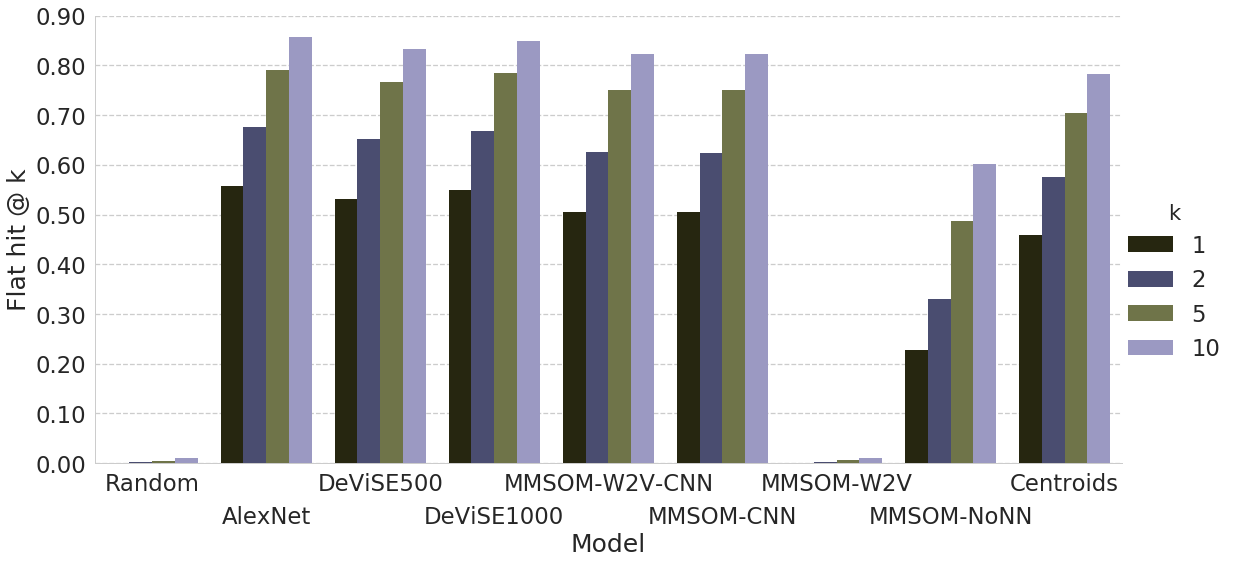
\includegraphics[width=\textwidth]{images/image_classification_results.png}
    \caption{ImageNet 1K Image classification experiment}
    \label{fig:ImageNet1KResults}
\end{figure}


\begin{table}[h]
    \begin{footnotesize}
        \begin{tabularx}{\textwidth}{|X|c|c|c|c|}
            \hline
            \multirow{2}{*}{Model} & \multicolumn{4}{ c|}{Flat hit @ $k$} \\
            \cline{2-5}            & 1               & 2               & 5               & 10        \\
            \hline
            Random guess           & 0.0010          & 0.0020          & 0.0050          & 0.0100    \\
            AlexNet\cite{krizhevsky2012imagenet}
                                   & \textbf{0.5565} & \textbf{0.6755} & \textbf{0.7906} & \textbf{0.8563}    \\
            DeViSE500\cite{frome2013devise}
                                   & 0.5320          & 0.6520          & 0.7670          & 0.8330    \\
            DeViSE1000\cite{frome2013devise}
                                   & 0.5490          & 0.6690          & 0.7840          & 0.8500    \\
            \hline
            MMSOM-W2V-CNN          & 0.5058          & 0.6249          & 0.7508          & 0.8233    \\
            MMSOM-CNN              & 0.5057          & 0.6247          & 0.7505          & 0.8234    \\
            MMSOM-W2V              & 0.0010          & 0.0020          & 0.0058          & 0.0111    \\
            MMSOM-NoNN             & 0.2279          & 0.3304          & 0.4867          & 0.6026    \\
            Centroids              & 0.4585          & 0.5764          & 0.7033          & 0.7821    \\
            \hline
        \end{tabularx}
    \end{footnotesize}
    \caption{ImageNet 1K Image classification experiment}
    \label{tab:ImageNet1KResults}
\end{table}

The results of our experiments for this section are presented in \figref{ImageNet1KResults}, and also in \tabref{ImageNet1KResults}, for a detailed reference. The models \verb|MMSOM-W2V-CNN|, \verb|MMSOM-CNN| and \verb|MMSOM-W2V| were trained and evaluated as described in \algref{TrainImgNetSOM, RetrieveImgNetLabel}. A schematic view of the network architecture used is shown in \figref{ImageNetExperimentArchitecture}. The \verb|Classifier| in the figure is a simple 3-layer, fully connected feed-forward NN, with 4396 input neurons, 4396 hidden neurons and 1000 output neurons. The reason for choosing this particular architecture was to introduce a non-linearity between the multi-modal embedding and the \verb|Softmax| layer in the \verb|Classifier|. Due to time constraints, we performed no hyper-parameter exploration.

Among \verb|MMSOM-W2V-CNN|, \verb|MMSOM-W2V| and \verb|MMSOM-CNN|, only \verb|MMSOM-W2V-CNN| was trained, whereas at test time:
\begin{itemize}
    \item \verb|MMSOM-CNN| has the input neurons corresponding to the GloVe embedding (green in the figure) in its classifier neural network zeroed out.
    \item \verb|MMSOM-W2V| has the input neurons corresponding to the image embedding (blue in the figure) in its classifier neural network zeroed out.
    \item \verb|MMSOM-W2V-CNN| works with both the image and GloVe embeddings.
\end{itemize}

\begin{figure}[h]
    \centering
    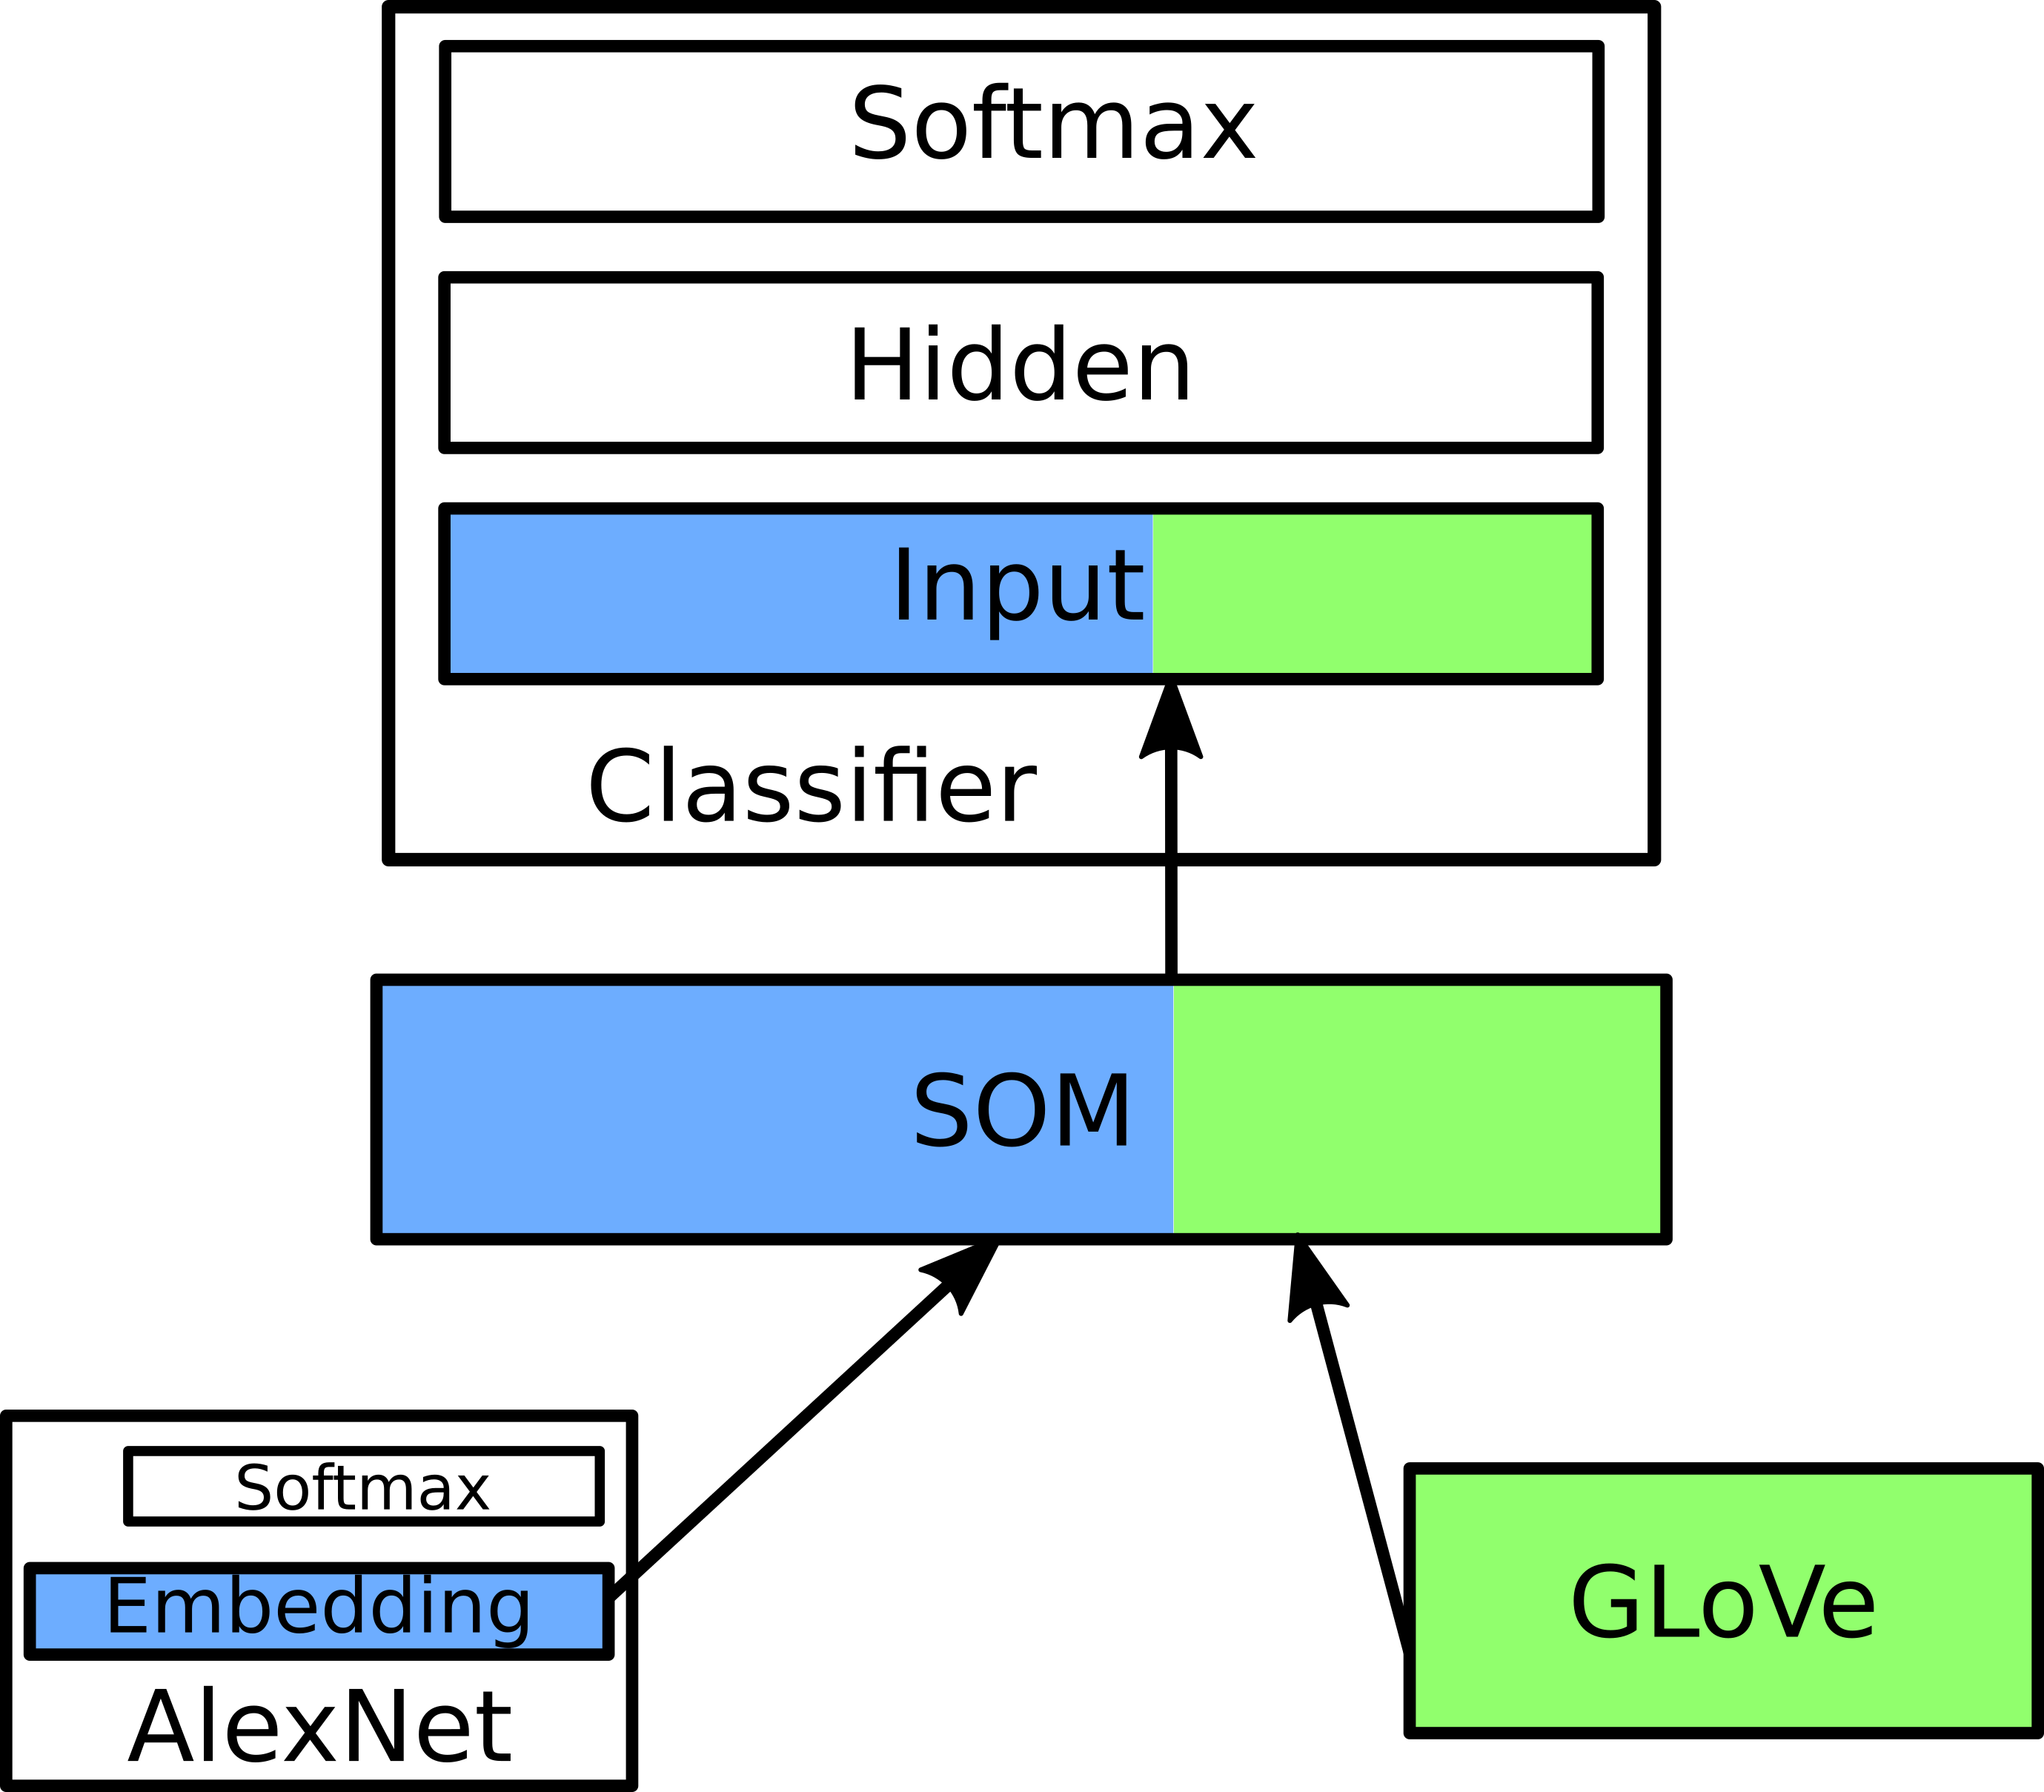
\includegraphics[width=0.5\textwidth]{images/ImageNetExperimentArchitecture.png}
    \caption{Network architecture for the Image classification Experiment. All layers in the Alex net model were used, except for the softmax layer. Blue indicates An image embedding, green indicates a word embedding.}\label{fig:ImageNetExperimentArchitecture}
\end{figure}

In contrast, \verb|MMSOM-NoNN| uses no classifier neural network. It relies instead on \algref{RetrieveWord}, with the 1000 object classes as its word search space, i.e., the \verb|w2vModel| contains in its vocabulary only the 1000 words corresponding to the object classes.

Finally, \verb|Centroids| uses neither SOM model nor classifier neural network. Its training consists on calculating and storing the mean image embedding for each object class in the training set; these form 1000 centroids. At test time, for each test image the nearest centroid to the test image is calculated, and the prediction is the label corresponding to that centroid. The method is explained in detail in \algref{RetrieveCentroidLabel}.

\begin{algorithm}[ht]
    \SetKwFunction{RetrieveCentroidLabel}{RetrieveImgNetLabel}
    \RetrieveCentroidLabel{$\Dcal_N$, $\vecx$}\\
    \KwData{
        $\Dcal_N = \{(\vecx_i, w_i); \vecx_i \in \Rbb^{M_1, M_2, 3}, w_i \in \Sbfs, i \in \Nbb_{\leq N}\}$: Dataset of image-word pairs. In this case, $\Sbfs$ consist of 1000 different words (training labels).\\
        $\vecx \in \Rbb^{M_1, M_2, 3}$: Image we want to retrieve an associated ImageNet label for.
    }
    \KwResult{$l_w \in \Rbb^{1000}$: encoded label associated with $\vecx$}
    \Begin{
        $\mathbf{cnnModel} \gets$ Load pre-trained AlexNet model.\;
        $centroids \gets (\Rbb^{1000\times 4096}, \Rbb^{1000})$\;
        \For{$w_i\ \mathbf{in}\ \Sbfs$}{
            $centroids[i, 0] \gets \mathbf{mean}(\{\mathbf{cnnModel.project}(\vecx_j): (\vecx_j, w_j) \in \Dcal_N \wedge w_j=w_i\})$\;
            $centroids[i, 1] \gets \mathbf{encodeLabel}(w_i)$\;
        }
        $cnnProj \gets \mathbf{cnnModel.project}(\vecx)$\;
        $nearestCentr \gets \arg \min_{c \in centroids} \Vert cnnProj - c[0] \Vert^2$\;
        $l_w \gets nearestCentr[1]$
    }
    \caption{Label prediction procedure for the ImageNet1K classification task using the \texttt{Centroids} approach.}\label{alg:RetrieveCentroidLabel}
\end{algorithm}

\subsection{Notes on \texttt{MMSOM-W2V-CNN} training}

Since we are dealing with 1000 words (object classes), we decided to use a square grid of $32\times 32 = 1024$ units for the SOM model. We hoped that, after training, at least one SOM unit would be associated with an object class. The SOM model was trained for 40 epochs, whereas the top NN model was trained for 100 epochs. These settings seemed sufficient for the NN classifier to converge to a minimum, therefore, we avoided optimizing the number of training epochs.

Several optimization methods were tried for the training of the \verb|Classifier| NN in \verb|MMSOM-W2V-CNN|: from plain stochastic gradient descent (SGD) to state-of-the-art approaches like Adam \cite{kingma2014adam}. Sadly, all adaptive methods failed to converge, being unable to improve on \textasciitilde 0.4 "flat hit @ 5" accuracy on the validation set. This is perhaps related to the work of Wilson et al. \cite{Wilson2017}. Therefore, we used plain SGD to train our final model.

We decided to use L1-regularization on the input layer and L2-regularization on the hidden layer. The idea was to analyze the relevance of the different embedding components on the classification. By using L1-regularization we aimed to induce sparsity in the input weights. Then, if the norm of a weight vector for a given input neuron is close to zero, this would mean that the input neuron was irrelevant to improving the accuracy of the model during training.

\subsection{Analysis and interpretation of results}\label{subsec:ImageClassificationAnalysis}

Although the performance of \verb|MMSOM-W2V-CNN| was lower than the DeViSE and AlexNet approaches, \verb|MMSOM-W2V-CNN| was close to them. This indicates that \verb|MMSOM-W2V-CNN| could be improved by a better training procedure (data augmentation, better optimization settings, etc.), or by alterations in the architecture. However, the extremely low impact of the GloVE embeddings on the training casts a doubt on whether the proposed approach was indeed useful. We expected the \verb|w2vModel| to provide extra information to the \verb|Classifier| NN, which was clearly not the case in practice.

Regarding the effects of the L1-regularization, from the 4096 input weight vectors for the CNN embedding in \verb|MMSOM-W2V-CNN|, 2056 had an euclidean norm lower than $10E^{-4}$ (~50\% of the vectors). In contrast, from the 300 input weight vectors for the GloVe embedding, 297 had an euclidean norm lower than $10E^{-4}$ (~99\% of the vectors). In other words, the GloVe embeddings had close to no influence on the training procedure. This concurs with the results from \tabref{ImageNet1KResults} for the \verb|MMSOM-W2V-CNN|, \verb|MMSOM-CNN| and \verb|MMSOM-CNN| models.

In contrast, \verb|MMSOM-NoNN| could present a better line of research. Even though it was behind both AlexNet and DeViSE, it was also far above the random guess baseline.

The \verb|Centroids| results gave us pause. They seem to imply that the images are clustered at the level of the CNN embedding, with each cluster corresponding to one ImageNet label, and with little overlap between clusters.
\end{document}